%!TEX root = main.tex

\section{Methodology}\label{methodology}

%We employed exploratory interviews with software practitioners and surveys of practitioners to validate our findings.

To understand the merge conflict processes, barriers, and resolution strategies of software developers, we used mixed methods consisting of interviews to gather qualitative insights, and surveys to provide quantitative triangulations into the broader context of merge conflicts.
Mixed methods allow us to identify perspectives and themes from both individual and population-wide samples to strengthen the validity of both, as per guidelines from Easterbrook et al.~\cite{easterbrook2008selecting}.

We conducted \textit{Exploratory Interviews} with software developers to create a taxonomy of processes, barriers, strategies, and concerns experienced by developers when encountering and resolving merge conflicts.
We then triangulate and extend the results of our interviews by conducting a \textit{Barriers Survey}~(S2) and a \textit{Processes Survey}~(S1) using concepts and vocabulary generated from the interviews. 

To analyze the scale of barriers, constraints, and concerns of software developers when approaching merge conflicts, we conducted a \textit{Barriers Survey}~(S2) of software developers.
In this survey, we sought to extend the results from our interviews and to include additional questions relating to tools, technology, and coordination within development teams.

Processes are developed to address common problems in teams and organizations.
Identifying the problems developers face is an essential element for process improvements~\cite{beecham2003software}.
We conducted an additional \textit{Processes Survey}~(S1) of software developers to understand how they monitor for merge conflicts, how they plan their resolution strategies, and their processes for evaluating whether their resolutions are successful.

The full set of questions in the interview, as well as the questions and codebooks used for both surveys can be found on our companion site~\footnote{Companion site: \url{http://engr.oregonstate.edu/~nelsonni/emse18.html}}.

\subsection{Exploratory Interviews}\label{interviews}

Semi-structured interviews provide qualitative data collection through open-ended questions that elicit interviewee's thoughts and opinions about a particular topic.
The resulting data includes themes and terminology from the perspective of the interviewee, as opposed to the interviewer, and provides a context for further quantitative inquiry~\cite{easterbrook2008selecting}.

We conducted semi-structured interviews with software developers to understand their concerns when facing merge conflicts and the factors that impact merge conflict difficulty.
We selected interview participants from top contributors to open-source projects, and from industry contacts using snowball sampling~\cite{goodman1961snowball} to reach a larger sample size. Additionally, we limited participant referrals to one connection per interviewee, where referred individuals did not provide additional referrals. In doing this, we sought to reduce the impact of any particular cohort of developers on the generalizability  of our results.

We interviewed ten software developers from seven different organizations spanning six different industries.
Eight of the participants worked primarily on open-source projects.
Participants worked on a variety of project sizes; from projects with less than five active contributors, to more than 1700 contributors (as evaluated by analyzing code repositories for a 12-month period).
Table~\ref{interview_demographics} provides additional demographics data, including software development experience, role, industry, project size, and whether the participant primarily focused on open- or closed-source software development.
Each interview lasted between 30 to 60 minutes.
Participants were offered US\$50 in either cash, gift card, or a donation to a charity of their choice.

\begin{table}[!htbp]
\renewcommand{\arraystretch}{1.3}
\caption{Interview Participant Demographics}
\label{interview_demographics}
\centering
\begin{tabularx}{\textwidth}{@{}llllrr@{}}
\toprule
	\parnoteclear % tabularx will otherwise add each note thrice
	\textbf{Par.}\parnote{Par. = Interview participant} & \textbf{Exp.}\parnote{Exp. = Years of software development experience} & \textbf{Role} & \textbf{Industry} & \textbf{Source}\parnote{Source = Source code licensing in primary project} & \textbf{\mbox{Contrib.}}\parnote{Contrib. = Approximate number of individual contributors in primary project (between March 2016-March 2017)\vspace*{-0.3\baselineskip}}\\
\midrule
	P1 & 18 yrs. & Sr. \mbox{Software} \mbox{Developer} & Semiconductor Mfr. & Open & 1700\\
	P2 & 6 yrs. & Software \mbox{Engineer} & Semiconductor Mfr. & Open & 1700\\
	P3 & 3 yrs. & Software \mbox{Engineer} & Semiconductor Mfr. & Open & 1700\\
	P4 & 10 yrs. & Software \mbox{Developer} & Academia & Open & \textless10\\
	P5 & 3 yrs. & Infrastructure \mbox{Engineer} & Healthcare Software & Closed & \textless10\\
	P6 & 5 yrs. & Software \mbox{Developer} & Healthcare Software & Closed & \textless10\\
	P7 & 5 yrs. & Software \mbox{Engineer} & Business Software & Open & 200\\
	P8 & 25 yrs. & Director & Academia & Open & 600\\
	P9 & 8 yrs. & Software \mbox{Developer} & IT Services & Open & 600\\
	P10 & 2 yrs. & Software \mbox{Developer} & Sports Software & Open & \textless5\\
\bottomrule
\end{tabularx}
\parnotes
\end{table}

At the beginning of the interview we gave participants a short explanation of the research goals, our definition of merge conflicts, and collected demographics data. 
We then asked participants about the roles that they play in their project, their experience working in team settings, questions about merge conflicts, the process of conflict resolution, and the difficulties that they faced in conflict resolution.

We formulated the interview questions about merge conflicts in order to understand how developers perceived and how they approached merge conflicts.
The following is an example of some of the questions we asked in the interview; the full set is available on our companion site.
\begin{itemize}
	\item Can you describe a merge conflict, or a set of conflicts, that you would consider to be the typical case?
	\item Do you have any particularly memorable merge conflict resolutions that you can recall?
	\item Have you had some code structures, design patterns, coding styles, etc., that you would consider a ``usual suspect'' in a conflict?
	\item What kind of measures would you take to minimize the amount of defects that you introduce?
\end{itemize}

The semi-structured interview format allowed participants to provide us with unanticipated information~\cite{seaman2008qualitative}. 
Further, we allowed open-ended discussion about merge conflicts in general at the end of the interview, which allowed participants to share ideas and topics that they found particularly important. 
We continued interviewing participants until we reached saturation in the answers, which was measured using topic saturation as our benchmark~\cite{fusch2015we}.

\subsection{Barriers Survey (S2)}\label{perceptions_survey}

In the initial survey step, we conducted a 50-question \textit{Barriers Survey} of software developers in order to examine the barriers, constraints, and concerns experienced when encountering merge conflicts.
We developed questions to confirm, extend, and broaden the results from the interviews.

\renewcommand*{\thefootnote}{\arabic{footnote}}
%\setcounter{footnote}{0}
We recruited participants from contributor lists on popular open-source repositories on GitHub, advertised on social networking sites (Facebook, Twitter and Reddit), and by directly contacting software developers via email. 
Participants spanned a variety of organization structures and geographical locations, giving generalizability to results.
The survey was conducted online and anonymity was guaranteed in order to elicit honest responses from participants.
The \textit{Barriers Survey}~(S2) was available for 56 days and we received 162 survey responses, but individual parts of the survey have varying response rates and are reported where appropriate in Section~\ref{results}.

Survey participants were given six different software roles to select, and in many cases, participants considered themselves to be fulfilling multiple roles. 
Table~\ref{survey_roles} provides a pairwise breakdown of participants' role selections, with a majority of participants considering themselves to be \textit{Software Engineer/Developer} (95.1\% overall).
Survey participants indicated a median software development experience of 6-10 years (36.4\% overall), and worked on project sizes ranging from 2 to more than 51 developers (the median was 2-5 developers, constituting 48.8\% of all responses).

\vspace*{-0.8\baselineskip}

\begin{table}[!htbp]
\caption{Barriers Survey (S2) Participant Roles\textsuperscript{i}}
\label{survey_roles}
\centering
\begin{tabularx}{\textwidth}{@{}r|*{10}{C}c@{}}
\toprule
\addlinespace[4.5em]
	& \begin{rotate}{30} Soft. Developers \end{rotate} 
	& \begin{rotate}{30} Sys. Architects \end{rotate} 
	& \begin{rotate}{30} DevOps \end{rotate} 
	& \begin{rotate}{30} Project Managers \end{rotate}
	& \begin{rotate}{30} Project Maintainers \end{rotate}
	& \begin{rotate}{30} Sys. Admins \end{rotate}
	& \begin{rotate}{30} Other \end{rotate}\\
\midrule
	Software Developers & 154 & & & & & & \\
	System Architects & 53 & 54 & & & & & \\
	DevOps & 51 & 34 & 53 & & & & \\
	Project Managers & 44 & 29 & 20 & 44 & & & \\
	Project Maintainers & 39 & 21 & 24 & 22 & 40 & & \\
	Systems Administrators & 22 & 16 & 15 & 14 & 12 & 23 & \\
	Other & 8 & 4 & 4 & 3 & 1 & 2 & 11 \\
\bottomrule
	\multicolumn{8}{c}{\noindent\parbox[t]{11.7cm}{\vspace{0.4em}\textsuperscript{i}\hspace{0.2em}\textit{Barriers Survey}~(S2) participants were allowed to select multiple roles. Each entry represents the number of participants that selected both of the roles indicated for the column and row. 62 out of 162 participants (38\%) selected three or more roles.}\vspace*{-0.3\baselineskip}}
\end{tabularx}
\end{table}

We divided the \textit{Barriers Survey}~(S2) into four categories, each category containing 5-7 questions (see our companion site for a list of questions).
First, we elicited background information about demographics, roles, and experience.
Second, we asked questions related to difficulties that developers experience when encountering merge conflicts.
Third, we asked questions related to conflict resolution and the factors that affect developers.
Finally we asked questions about the tools and tool features that developers use when working with merge conflicts.
Questions were presented either as 5-point Likert-type scales (with no pre-selected answers) or open-ended text forms to gather additional insights.

\subsection{Processes Survey (S1)}\label{processes_survey}

Merge conflicts disrupt the collaborative development workflow, and developers have adapted and developed different processes for handling these complexities.
To understand the common structure and prevalence of these processes we use surveys, which are used for mapping the state of practice, establishing baselines for investigating research topics, and gathering opinions regarding software engineering technologies and practices~\cite{deMello2016survey}.
Therefore, we conducted a second 15-question \textit{Processes Survey} (S1) of software developers that included both open-ended and predefined questions.

We recruited participants for \textit{Processes Survey}~(S1) to be similar to \textit{Barriers Survey}~(S2) participants so that we could compare and triangulate the results.
We therefore recruited participants from contributor lists on popular open-source repositories on GitHub, advertised on social networking sites (Twitter and Reddit), and by directly contacting software developers via email.
Due to the nature of social media and mailing lists, we cannot compute a response rate from these distribution methods.
We observe that 35.29\% of participants were located outside of the United States and several participants indicated that they sent the survey onward to other software developers.

The survey was conducted online and anonymity was guaranteed.
The \textit{Processes Survey}~(S1) was available for 38 days and we received 113 survey responses, however, 11 responses were incomplete, resulting in 102 total responses.
The results of this survey are presented in Section~\ref{results}.

%\begin{figure}[!htbp]
%\centering
%\hspace*{-0.7cm}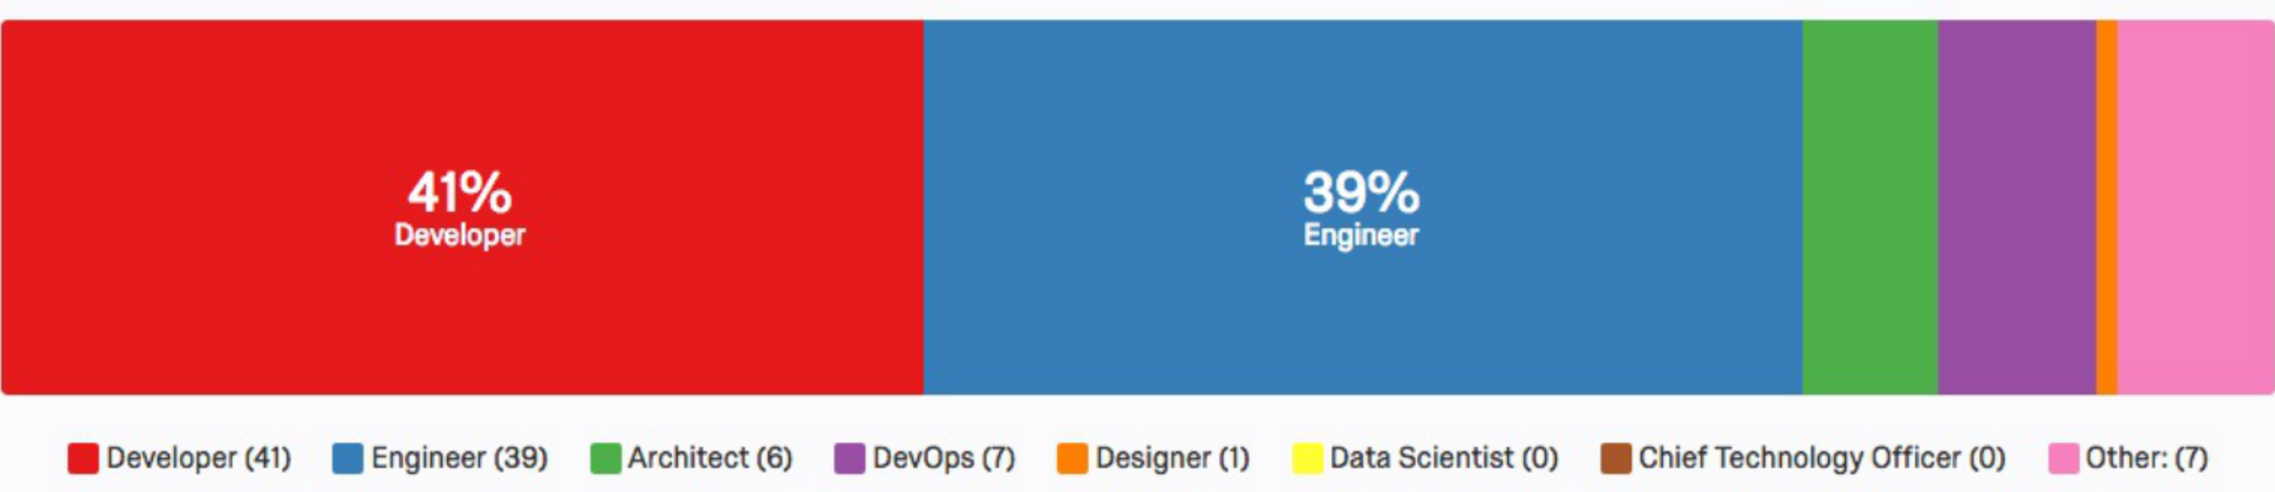
\includegraphics[width=1.105\textwidth,keepaspectratio]{ProcessesParticipantRoles}
%\caption{Distribution of primary roles from Processes Survey~(S1) participants: 45.5\% are primarily a \textit{Developer}, 42.0\% an \textit{Engineer}, 12.5\% \textit{Other}, and 12.8\% were either \textit{DevOps}, \textit{Architect}, or \textit{Designer}. No participants selected \textit{Data Scientist} or \textit{Chief Technology Officer}.\vspace*{-0.3\baselineskip}}
%\label{processes_roles}
%\end{figure}

\newcolumntype{Y}{>{\centering\arraybackslash}X}

\begin{table}[!htbp]
\renewcommand{\arraystretch}{1.3}
\caption{Distribution of primary roles from Processes Survey~(S1) participants}
\label{processes_roles}
\centering
\begin{tabularx}{\textwidth}{@{}YY@{}}
\toprule
	\textbf{Job Title} & \textbf{Response Rate}\\
\midrule
	Developer & 45.5\%\\
	Engineer & 42\%\\
	Other & 12.5\%\\
	DevOps & 6.9\%\\
	Architect & 5.0\%\\
	Designer & 1.0\%\\
	Data Scientist & 0\%\\
	Chief Technology Officer & 0\%\\
	
\bottomrule
\end{tabularx}
\end{table}

Survey participants had a mean of 9.1 years of programming experience, and primarily worked in teams of 2-5 members (45.10\% overall).
Participants were assumed to be software developers in some capacity, but primary roles within individual organizations can differ throughout the industry.
Participants were given seven different roles to select, as well as an \textit{Other} field to provide additional roles not included in the pre-populated options.
Table~\ref{processes_roles} provides a visual illustration of the distribution of primary roles among participants.
87.5\% of participants were primarily a \textit{Developer} or \textit{Engineer} (45.5\% and 42.0\% respectively), with 6.9\% selecting \textit{DevOps}, 5.0\% \textit{Architect}, 1.0\% \textit{Designer}, and 12.5\% \textit{Other}.
Among participants that selected \textit{Other}, the open-text responses included: ``Tester,'' ``Security Analyst,'' ``Hobbyist Programmer,'' and ``Researcher.''

We divided the survey into four categories, with each containing 3-5 questions (see \cite{companion_site} for individual questions).
First, we elicited background information about demographics, roles, and experience.
Second, we asked questions relating to how and when developers become aware of merge conflicts.
Third, we asked questions related to planning and implementing merge conflict resolution strategies.
Finally, we asked questions about evaluating the effectiveness of those merge conflict resolutions and the particular tools that are used throughout the processes of working with merge conflicts.

\subsection{Data Analysis}\label{analysis}
To ensure that our survey samples are representative of the larger developer population, we compare the demographics from the \textit{Processes Survey}~(S1) and the \textit{Barriers Survey}~(S2) with the results of the 2018 StackOverflow Developer Survey\footnote{https://insights.stackoverflow.com/survey/2018}.

The 2018 StackOverflow Developer Survey was conducted on 101,592 software developers from 183 countries.
This survey includes the number of years spent coding professionally by 77,903 participants.
%, and is presented as totals for buckets of 0-2 years, 3-5 years, 6-8 years, 9-11 years, 12-14 years, 15-17 years, 18-20 years, 21-23 years, 24-26 years, 27-29 years, and 30 or more years.
%For comparison purposes, we similarly grouped the results from the \textit{Processes Survey}~(S1) and the \textit{Barriers Survey}~(S2).
Figure~\ref{populations} provides a graphical representation of the percentile distribution of professional programming experience among participants in the \textit{Processes Survey}~(S1), \textit{Barriers Survey}~(S2), and the 2018 StackOverflow Developer Survey.
We see that our sample population has more experienced developers, and the trends match between all three samples.

\begin{figure}[!htbp]
\centering
\fbox{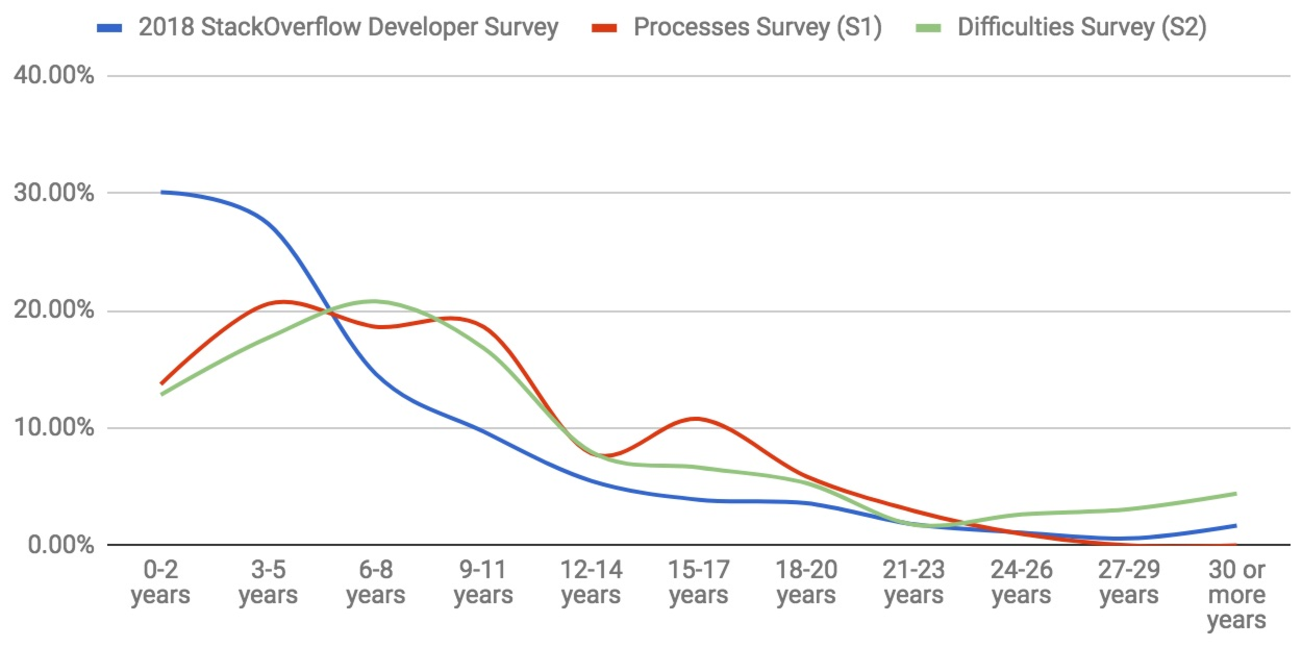
\includegraphics[width=0.98\textwidth,keepaspectratio]{imgs/populations}}
\caption{Percentile distributions of professional programming experience compared between \textit{Processes Survey}~(S1), \textit{Barriers Survey}~(S2), and 2018 StackOverflow Developer Survey participants. Responses are inclusively binned into 3-year buckets for comparison across surveys.\vspace*{-0.3\baselineskip}}
\label{populations}
\end{figure}

To further compare the distribution of programming experience across these population samples, we conduct nonparametric tests of the equality of the probability distributions between two samples.
Comparing \textit{Processes Survey}~(S1) responses with 2018 StackOverflow Developer Survey responses, we conclude that we cannot reject the null hypothesis that these samples were drawn from the same population distribution (Two-sample Kolmogorov-Smirnov test, $D = 0.33636$, p-value$ = 0.5939$).
We similarly conclude that \textit{Barriers Survey}~(S2) responses and 2018 StackOverflow Developer Survey responses could plausibly be drawn from the same population distribution (Two-sample Kolmogorov-Smirnov test, $D = 0.27273$, p-value$ = 0.8326$).
In both cases, we cannot reject the null hypothesis that the survey sample population is the same as the 2018 StackOverflow Developer Survey population, therefore, we conclude that our samples are representative of the development community.

\subsubsection{Interview Analysis}

Interviews were audio-taped and transcribed. 
The first and third authors unitized~\cite{unitization} the interview transcripts into cards that each contained a single logically consistent statement. 
To organize these cards we employed card sorting, a collaborative technique of exploring how people think about a certain topic~\cite{spencer2009card,card_sort}, which allows key concepts and associations to be identified through an open sorting method that iteratively develops categories during the process.

We performed two iterations of the open card sorting process.
In the first iteration, we developed a standardized coding scheme and improved it to an acceptable point through \textit{negotiated agreement,} which was reached when no further thematic categories could be created and agreed upon by both coders~\cite{garrison2006revisiting,ritchie2013qualitative}.
The coding scheme dictated that sentences must be consecutive and topically related to be grouped into a single card.
Logically connected statements that were separated by other lines were considered to be separate cards, as a conservative measure to preserve context within each card.

In the second iteration, the first and third authors sorted cards according to our coding scheme and discussed the resulting taxonomies until consensus was reached.
Based upon our research questions, we grouped the resulting categories as follows: the processes that developers use for merge conflicts (Section~\ref{RQ1}, the difficulties that developers face with merge conflicts (Section~\ref{RQ2}), and the impact of development tools on the resolution process (Section~\ref{RQ3}).

\subsubsection{Survey Analysis}

We evaluated the results of the \textit{Barriers Survey}~(S2) by performing open card sorting on the all open-ended questions.
The resulting categories were standardized to an acceptable point through \textit{negotiated agreement}~\cite{ritchie2013qualitative}.

The \textit{Barriers Survey}~(S2) was primarily composed of Likert-type questions, which were used to measure the extent to which participants agreed with a particular statement.
This means that lower mean and median values indicate less agreement with the statement in a particular question.
We use this design to validate both the degree of agreement to the interview results, as well as the existence of individual factors.

We present the results of the \textit{Exploratory Interviews,} \textit{Processes Survey}~(S1) and \textit{Barriers Survey}~(S2) in Section~\ref{results}.
When necessary, we refer to individual survey participants by a combination of the survey short-hand (S1 or S2) and participant number; for example S1--14 is participant 14 from the \textit{Processes Survey}~(S1) responses.

For the \textit{Processes Survey}~(S1), we evaluated the distribution of survey answers for each of the four Likert-type question by analyzing across demographic categories.
We used Likert-type questions to measure the extent to which participants agreed with a particular statement, or the degree to which a factor has impacted the participant.
Where answers differed across a demographic category, we note the difference and provide further discussion of these results.

The \textit{Processes Survey}~(S1) contained five open-ended questions.
We performed open thematic coding~\cite{fereday2006demonstrating} to analyze the responses to these questions.
The resulting codebook, including descriptions and examples, are available on our companion site.
%Table~\ref{tab:codes} provides the resulting codebook, including descriptions and examples.
After establishing a codebook, the first two authors independently coded the responses to each open-ended question.
For question 7 (\textit{``How do you monitor for merge conflicts?''}), we achieve an inter-rater reliability (IRR) agreement of $0.95$ (Jaccard similarity coefficient).
For questions 8 (\textit{``How do you determine the urgency of a merge conflict?''}), 11 (\textit{``What is your first step in trying to understand code involved in a merge conflict?''}), 14 (\textit{``What effect did deferring your response to a merge conflict have on the resolution of the conflict?''}), and 19 (\textit{``If your first attempt at resolving a merge conflict fails, what backup strategies do you use?''}), we achieve IRR agreements of $0.81$, $0.88$, $0.74$, and $0.92$, respectively (all are above the Software Engineering research standard of $0.80$ IRR).

%\def\shift{\hspace{0.5em}}
%\begin{table}[!htbp]
%\centering
%\caption{Codebook used for coding open-ended responses from Processes Survey (S1)}
%\label{tab:codes}
%\begin{tabular}{lp{1.5in}p{1.3in}}
%\toprule
%Code & Description & Example \\
%\midrule
%\multicolumn{3}{l}{\textbf{Q7: How do you monitor for merge conflicts?}} \\
%\shift Proactive & & \\
%\shift Reactive & & \\
%\midrule
%\multicolumn{3}{l}{\textbf{Q8: How do you determine the urgency of a merge conflict?}} \\
%\shift Project Structure & & \\
%\shift Code Under Conflict & & \\
%\shift External Dependencies & & \\
%\shift No System & & \\
%\midrule
%\multicolumn{3}{p{4.5in}}{\raggedright\textbf{Q11: What is your first step in trying to understand code involved in a merge conflict?}} \\
%\shift About the conflict & & \\
%\shift The Code Itself & & \\
%\shift Analyzing the code & & \\
%\shift Design Concerns & & \\
%\shift Project Organization & & \\
%\shift No-op & & \\
%\midrule
%\multicolumn{3}{p{4.5in}}{\raggedright\textbf{Q14: What effect did deferring your response to a merge conflict have on the resolution of the conflict?}} \\
%\shift Physical Manifestations & & \\
%\shift External to company impact & & \\
%\shift Policy/culture changes & & \\
%\shift The Nuclear Option & & \\
%\shift Increased Complexity & & \\
%\shift Stop the presses & & \\
%\shift No-op & & \\
%\midrule
%\multicolumn{3}{p{4.5in}}{\raggedright\textbf{Q19: If your first attempt at resolving a merge conflict fails, what backup strategies do you use?}} \\
%\shift Collaborating & & \\
%\shift Redoing changes & & \\
%\shift Take it offline & & \\
%\shift Try again & & \\
%\shift No strategy/Other & & \\
%\bottomrule
%\end{tabular}	
%\end{table}